% !TEX root =  master.tex
\cleardoublepage
\chapter{PCR-Pooling}
\section{Parameter und Kenngrößen}

Die \textbf{Prävalenz} ist die Quote, mit welcher eine Krankheit in einer Bevölkerungsgruppe auftritt.\footcite{gordis_epidemiologie_2001}%[S37]
Sie ist ähnlich dem Konzept der Inzidenz, welche sich auf die Gesamtbevölkerung bezieht.
Bei einer anlassbezogenen Testung werden meist deutlich höhere Prävalenzen beobachtet.
Gemäß RKI-Wochenbereicht sind zwischenzeitlich über 40 Prozent der PCR-Tests positiv.\footcite{noauthor_rki-bericht_2021}

Das PCR-Verfahren ist darauf ausgelegt, geringe DNA-Mengen zu einer nachweisbaren Menge zu vermehren.
Die Verwässerung der Probe ist deshalb bis zu einem gewissen Punkt unproblematisch für den Nachweis.
Hierdurch wird ein \textbf{Pooling} von mehreren Testpersonen möglich.
Die Proben der Patienten werden zunächst zu einem Pool zusammengefasst und anschließend gemeinsam getestet.

Das Verfahren funktioniert grundsätzlich auch bei hoher Verdünnung.
Die Erkennungsrate sinkt hierbei allerdings.
Eine Grenze bis zu welchem Punkt das Verfahren funktioniert, gibt es nicht.
Das Verfahren verliert mit zunehmender \textbf{Verwässerung} stufenlos an Genauigkeit.
Abgewogen werden muss deshalb zwischen Präzision und Kostenersparnis.

Eine Poolgröße von bis zu 20 Personen ist laut Viehweger "comfortable above the detection rate"\footcite{viehweger_increased_2020}
Andere Gruppe halten Poolgrößen von bis zu 90 Personen für akzeptabel.\footcite{verwilt_evaluation_2021}
Es ist zu beachten, dass bei größeren Pools mehr Verdopplungsschritte notwendig sind, um dieselbe Virenmenge in der Probe zu erhalten.
Beim Pooling von 16 Personen liegt beispielsweise eine um $2^{4}$ niedrigere Virenlast vor.
Deshalb müssen 4 weitere Zyklen eingeplant werden.\footcite{viehweger_increased_2020}

\cleardoublepage

\section{Umgang mit dem Ergebnis}
\begin{itemize}
	\item Ein \textbf{Negatives Poolergebnis}
	bedeutet, dass \textbf{jede Einzelprobe negativ} war.
	Es wurde somit durch einen Test festgestellt, dass alle Personen im Pool negativ sind.
	
	\item Ein \textbf{Positives Poolergebnis} bedeutet, dass \textbf{mindestens eine Einzelprobe positiv} war.
	In diesem Fall müssen weitere Tests durchgeführt werden, um die positiven Einzelpersonen zu ermitteln.
\end{itemize}

\begin{figure}[h]
	\centering
	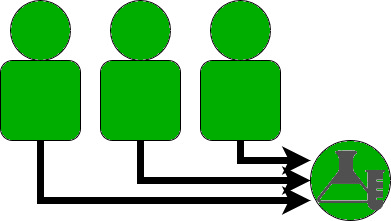
\includegraphics[width=.5\textwidth]{img/PoolAlleNegativ}
	\caption{Pooling benötigt für drei negative Personen nur ein Test\footnotemark}
\end{figure}

\footnotetext{Eigene Darstellung}



\textbf{Unklare Ergebnisse}\newline
Durch Pooling besteht das Risiko, dass die Ergebnisse nicht für alle Testpersonen eindeutig interpretiert werden können.\footcite{viehweger_increased_2020}
Wie häufig dies der Fall ist und welcher Anteil der Testgruppe nachuntersucht werden muss, ist abhängig von den gewählten Parametern.

\begin{figure}[h]
	\centering
	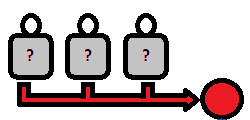
\includegraphics[width=.5\textwidth]{img/PoolPositiv}
	\caption{Ein positiven Pool kann die positive Person nicht identifizieren\footnotemark}
\end{figure}
\footnotetext{Eigene Darstellung}

Hierdurch werden \textbf{Nachtestungen} der betroffenen Personen notwendig.
Die Tests erfolgen hierbei nacheinander und sind statistisch unabhängig voneinander.
Manche Methoden erfordern sogar mehrere sequenzielle Nachtestungen.\footcite{verwilt_evaluation_2021}

Um Nachtestungen zu ermöglichen, müssen die Proben ausreichend Substanz für mehrere Testungen enthalten.
Durch die erneute Testung verlängert sich der Zeitraum, bevor für alle Testpersonen das Ergebnis fest steht.

Beim ersten Poolingdurchlauf muss darauf geachtet werden, die Proben untereinander nicht zu kontaminieren.
Eine Verunreinigung der Originalproben würde eine spätere Nachtestung unmöglich machen.\footcite{verwilt_evaluation_2021}
Um eine \textbf{Kontamination} durch das Pooling zu verhindern, sollte die komplette Matrix vor dem Pooling einmal dupliziert werden. 
Die für den aktuellen Test notwendigen Proben werden hierbei entnommen und im Duplikat gepoolt.
Für diesen Duplikationsschritt gibt es spezialisierte Laborgeräte, sodass dies in einem Arbeitsschritt für alle Proben durchgeführt werden kann - teilweise sogar automatisiert.\footcite{kendall_antigen-based_2021}

\begin{figure}[h]
	\centering
	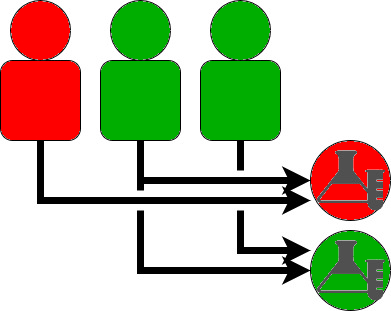
\includegraphics[width=.4\textwidth]{img/KomplexePools}
	\caption{Überlappende Pools\footnotemark}
\end{figure}
\footnotetext{Eigene Darstellung}

\textbf{Überlappende Pools}\newline
Um das Problem der Nachtestungen zu lösen, kann man mehrere überlappende Tests durchführen.
Aus der Kombination der Ergebnisse ist es theoretisch möglich, die infizierte Person zu triangulieren.\footcite{verwilt_evaluation_2021}

Schwierig wird es hierbei, wenn mehrere Personen innerhalb der Testgruppe positiv sind.
Die positiven Tests lassen sich dann nicht mehr exakt einer Person zuordnen.\footcite{viehweger_increased_2020}
\cleardoublepage

\begin{figure}[h]
	\centering
	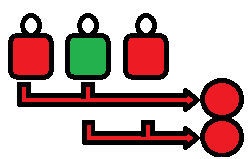
\includegraphics[width=.4\textwidth]{img/MehrerePositiv}
	\caption{Mehrere Positivfälle\footnotemark}
\end{figure}
\footnotetext{Eigene Darstellung}
Das Ergebnis in Abbildung 3.4 legt nahe, dass die mittlere Person infiziert ist.
Beide Pools fallen positiv aus und nur die mittlere Person ist Teil beider Testgruppen.
Für diese Person wäre es somit naheliegend ein falsch-positives Ergebnis mitzuteilen.

Die Kosten der Testung erhöhen sich zudem für alle Testgruppen, da durch diese Strategie für die erste Testrunde bereits zwei Tests notwendig sind, um eine Testgruppe von drei Personen abzubilden.

\begin{figure}[h]
	\centering
	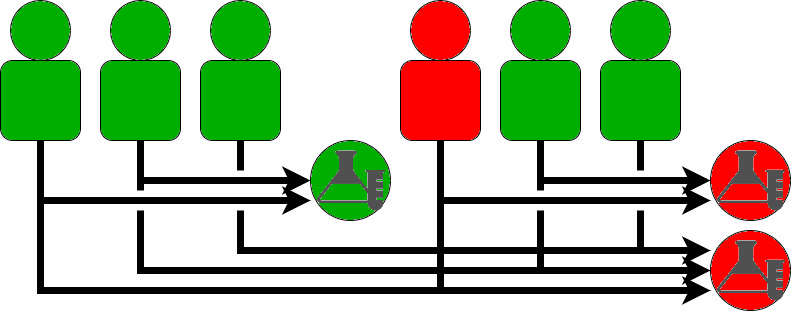
\includegraphics[width=.8\textwidth]{img/GrossePooluebersicht}
	\caption{Überlappende Pools\footnotemark}
\end{figure}
\footnotetext{Eigene Darstellung}

Weitere Schwierigkeiten ergeben sich, wenn für Personen gemischte Ergebnisse vorliegen.
In Abbildung 3.5 sind bei den drei Personen der rechten Testgruppe beide Pooltests positiv ausgefallen.
In dieser Gruppe sind höchstwahrscheinlich eine oder mehrere Personen infiziert und die Gruppe muss nachgetestet werden.

Bei den Personen der linken Gruppe liegt allerdings ein positives und ein negatives Ergebnis vor.
Theoretisch kann durch das negative Ergebnis ausgeschlossen werden, dass eine Person dieser Gruppe infiziert ist.
In der Praxis ist allerdings kein Test 100 Prozent zuverlässig.\footcite{verwilt_evaluation_2021}
Für diese Personen liegt somit ein positiver Pool vor und das Negativergebnis könnte fehlerhaft sein.
Testet man nun zur Sicherheit nochmal alle?

Die \textbf{sicherste Variante} wäre, alle Personen nachzutesten die Teil eines positiven Pools waren.
Hierdurch wäre der Mehrwert durch das Pooling allerdings schnell verloren.
Abhängig vom Anwendungsfall kann es dagegen akzeptabel sein, einige Infektionen nicht zu erkennen.\footcite{weishampel_orasure_2022}
Dies ist bei anlasslosen Massentestungen der Fall sein in denen kein Negativzertifikat ausgestellt wird.
Die Kostenoptimierung steht hierbei im Vordergrund, sodass \textbf{einige falsch-negative Ergebnisse akzeptabel} sein können. 

In der Praxis sollte meist ein Mittelweg gewählt werden.
Dieser könnte beispielsweise sein, alle mutmaßlich negativen Personen einer Testgruppe in einem gemeinsamen Pool nachzutesten.
Dieser Pool hat damit eine erwartete Prävalenz von null und sollte immer negativ ausfallen.
Hierdurch kann ermittelt werden, ob beim ersten Durchlauf Fehler passiert sind und Personen übersehen wurden.
Sollte dieser Pool positiv werden, müssen alle Teilnehmer einzeln nachgetestet werden.
Hierduch werden bereits drei sequenzielle Durchläufe notwendig
Die Übermittlung des Testergebnisses wird hierdurch stark verzögert, was ebenfalls Probleme verursachen kann.\footcite{viehweger_increased_2020}

\section{Ermittlung des Erwartungswertes}
Als \textbf{Effizienz} einer Poolingmethode wird nachfolgend der Multiplikator bezeichnet, welcher gegenüber Einzeltestungen erzielt werden kann.\footcite{viehweger_increased_2020}
Diese ist Abhängig von der Größe der Testgruppe und der Anzahl der Tests die erforderlich sind, um den Infektionsstatus jeder Person zu klassifizieren.
Die Effizienz lässt sich somit beschreiben als $\frac{Anzahl Testpersonen}{Anzahl Tests} $.
\begin{figure}[h]
	\centering
	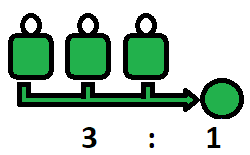
\includegraphics[width=.4\textwidth]{img/EffizienzNegativ}
	\caption{\mbox{Effizienz eines} \mbox{negativen} Pools\footnotemark}
\end{figure}
\footnotetext{Eigene Darstellung}
Im bestmöglichen Fall ist die gesamte Testgruppe nicht infiziert.
Hierdurch fallen im ersten Durchlauf alle Tests negativ aus und die gesamte Testgruppe kann als negativ markiert werden.
Im Beispiel der Abbildung 3.6 ergibt sich eine Effizienz von 3,0.

Bei einem positiven Pool wird zunächst ein Pooltest benötigt und danach ein Einzeltest für jede Person.
Die Effizienz lässt sich somit beschreiben als $\frac{Anzahl Testpersonen (N)}{1 Pooltest + N Einzeltests} $.
Für Abbildung 3.7 liegt die Effizienz damit bei 0,75 und ist schlechter, als wenn direkt einzeln getestet worden wäre.

\begin{figure}[h]
	\centering
	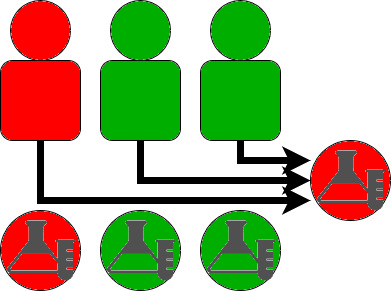
\includegraphics[width=.4\textwidth]{img/EffizienzPositiv}
	\caption{\mbox{Effizienz eines} \mbox{positiven Pools}\footnotemark}
\end{figure}
\footnotetext{Eigene Darstellung}

Der \textbf{Erwartungswert für die Effizienz} kann als Kennzahl für die Bewertung von Teststrategien eingesetzt werden.
Die benötigte Anzahl der Tests ist abhängig vom Ergebnis der Pooltests.
\begin{itemize}
	\item \textbf{Alle Ergebnisse negativ:} Keine Nachtestungen. Effizienz 3,0. 
	\item \textbf{Poolergebnis positiv:} Einzelne Nachtestungen. Effizienz 0,75.
\end{itemize}
Der Erwartungswert ergibt sich aus diesen beiden Szenarien, gewichtet nach ihrer Eintrittswahrscheinlichkeit.
Die Wahrscheinlichkeit, dass jemand innerhalb der Testgruppe Infiziert ist, hängt von der Prävalenz und der Größe der Testgruppe ab.
\cleardoublepage
